%=============================================================================
% MIA 5100 — Snap-to-Sell — Final Report (IEEE conference format)
% Build:  pdflatex final_report_5pg -> bibtex final_report_5pg -> pdflatex x2
% Needs IEEEtran.cls and IEEEtran.bst (TeX Live / MacTeX).
% Target length: 5 pages.
%=============================================================================
\documentclass[conference]{IEEEtran}

\usepackage{cite}
\usepackage{url}
\usepackage{amsmath,amssymb,amsfonts}
\usepackage{graphicx}
\usepackage[hidelinks]{hyperref}
\usepackage{array}
\usepackage{booktabs}
\usepackage{textcomp}
\usepackage{xcolor}
\usepackage{microtype}

\graphicspath{{figures/}}
\usepackage{tikz}
\usetikzlibrary{shapes.geometric,arrows.meta,positioning}

\tikzstyle{block}=[
draw,
rounded corners,
minimum width=2.8cm,
minimum height=1cm,
text centered,
fill=blue!8
]

\tikzstyle{arrow}=[
thick,
->,
>=Stealth
]

\begin{document}

\title{Snap-to-Sell: An Open-Source Pipeline for Turning a Corner-Store
Product Photograph into a Retrieval-Grounded E-Commerce Listing}

\author{%
\IEEEauthorblockN{1\textsuperscript{st} Ikenna Okonkwo}
\IEEEauthorblockA{\textit{University of Ottawa}\\
Ottawa, ON, Canada\\
iokon081@uottawa.ca}
\and
\IEEEauthorblockN{2\textsuperscript{nd} Loic Tiemani}
\IEEEauthorblockA{\textit{University of Ottawa}\\
Ottawa, ON, Canada\\
ltiem089@uottawa.ca}
\and
\IEEEauthorblockN{3\textsuperscript{rd} Frank Boahen}
\IEEEauthorblockA{\textit{University of Ottawa}\\
Ottawa, ON, Canada\\
fboah074@uottawa.ca}
\and
\IEEEauthorblockN{4\textsuperscript{th} Mou Rani Adhikary}
\IEEEauthorblockA{\textit{University of Ottawa}\\
Ottawa, ON, Canada\\
madhi020@uottawa.ca}
}

\maketitle

%------------------------------------------------------------------------------
\begin{abstract}
Independent retailers increasingly sell inventory through online marketplaces,
but onboarding products is labor-intensive because each listing requires
product identification, pricing, imagery, category assignment, and description
generation. We present Snap-to-Sell, an open-source pipeline that transforms a
single smartphone photograph of a packaged retail product into a draft
e-commerce listing. The system combines vision-language reasoning, packaging
OCR, retrieval-grounded product search, automated listing generation,
catalogue-image verification, and responsible-AI safeguards. On a hand-labelled
dataset of 58 retail products spanning food, beverage, household,
personal-care, tobacco, and alcohol categories, Snap-to-Sell improved over a
naive vision-language baseline on four of six measured dimensions, achieving
86.2\% top-1 identification accuracy, 79.3\% category accuracy, 100\%
age-restricted-item recall, and upgrading 29.3\% of product images. Price
estimation remained the system's primary limitation, driven by retrieval
ambiguity and multipack matching errors. These results suggest that
retrieval-grounded multimodal systems can meaningfully reduce listing effort
while preserving transparency, traceability, and human oversight.
\end{abstract}

\begin{IEEEkeywords}
computer vision, vision-language models, e-commerce, retrieval augmented
generation, product recognition, responsible artificial intelligence
\end{IEEEkeywords}

%------------------------------------------------------------------------------
\section{Introduction}

The growth of e-commerce has transformed how products are discovered and sold.
Large retailers maintain sophisticated product-information systems and dedicated
catalogue teams, whereas independent convenience stores rely on manual processes
for inventory digitization. Creating a single listing requires identifying the
product, researching pricing, selecting images, assigning categories, and
writing descriptions; effort that scales poorly across hundreds of products and
forms a major barrier to digital adoption.

Recent advances in multimodal AI create opportunities to automate these tasks.
Vision-language models (VLMs) such as CLIP demonstrate strong zero-shot
recognition by learning aligned visual and textual representations from
large-scale image-text data \cite{radford2021clip}, while retrieval-grounded
generation improves factual consistency by conditioning language models on
external evidence \cite{li2024modict}. Retail datasets such as RP2K and CAPG-GP
show that fine-grained product identification is achievable with modern
multimodal approaches \cite{peng2020rp2k,geng2018oneshot}. This project targets
packaged consumer products: food, beverages, household goods, personal care,
tobacco, and alcohol. Rather than proposing a novel model, it investigates
whether existing AI systems and public data sources can be integrated into a
reliable workflow that turns one product photograph into a publishable listing.

Product onboarding remains largely manual, and practical deployment requires far
more than recognition. Many packaged products are visually similar and differ
only in flavour, size, or regional variation \cite{peng2020rp2k}; retrieval
systems often return multipacks or bundles, creating pricing errors
\cite{llp2025}; language models can generate unsupported claims without external
grounding \cite{li2024modict}; and regulated items such as alcohol and tobacco
add compliance requirements. A practical solution must therefore prioritize
trustworthiness, transparency, and human oversight rather than automation alone.

\textbf{Research question.} \textit{How accurately can a vision-language and
retrieval pipeline identify packaged corner-store products from a single image
and generate a publishable, correctly priced listing, and where does it
systematically fail?} To answer this, we (i) build an end-to-end pipeline that
converts a photograph into a structured listing; (ii) quantify performance
across identification, pricing, listing quality, image upgrade, and
responsible-AI metrics; (iii) characterize failure modes including look-alike
products, multipack ambiguity, and restricted-item handling; and (iv) integrate
responsible-AI safeguards that detect age-restricted products, flag unsupported
claims, and route uncertain predictions to review.

Our contributions are: a fully integrated, openly documented pipeline; the
fusion of VLM reasoning with packaging OCR to improve recognition
\cite{ocrfusion2023}; retrieval-grounded metadata generation from public product
databases \cite{li2024modict}; catalogue-image verification via visual
similarity and perceptual hashing \cite{sir2020,eclip2022}; and integrated
responsible-AI safeguards spanning confidence estimation, age-restriction
detection, grounding verification, and human-in-the-loop review.

%------------------------------------------------------------------------------
\section{Literature Review}

Automated retail-listing generation sits at the intersection of retail product
recognition, vision-language modelling, retrieval-augmented generation, price
estimation, product-image retrieval, and responsible AI. Substantial progress
exists within each area, but little work evaluates a unified workflow that turns
a product photograph into a publishable listing.

\textit{Recognition and vision-language models.} Retail recognition is a
fine-grained classification problem: systems must separate products with nearly
identical appearance, small packaging differences, and shifting assortments.
Benchmarks such as RP2K and CAPG-GP establish this difficulty under real-world
imaging conditions \cite{peng2020rp2k,geng2018oneshot}. Supervised classifiers
struggle with unseen products and require continual retraining, so recognition
has shifted toward VLMs such as CLIP, which enable zero-shot classification and
semantic retrieval without task-specific training \cite{radford2021clip}.
Because many packaged goods differ chiefly through printed text ("Diet",
"Zero Sugar", "Family Size" flavours), image-only reasoning is
insufficient, motivating fusion with OCR-derived features \cite{ocrfusion2023}.

\textit{Retrieval grounding, pricing, and imagery.} Retrieval-augmented
generation improves factual consistency by grounding outputs in external
evidence, making generated titles, descriptions, and prices traceable and
auditable \cite{li2024modict}. Pricing is difficult because values vary by
store, location, promotion, and package configuration; direct regression from
images or text \cite{chen2018priceright} offers limited transparency, whereas
retrieval-grounded pricing derives estimates from observed comparables but is
dominated by retrieval quality, with multipacks and bundles a persistent source
of error \cite{llp2025}. For imagery, similarity-learning systems such as SIR
and e-CLIP identify semantically equivalent products across viewpoint and
lighting differences, but require same-SKU verification before replacement to
avoid incorrect substitutions \cite{sir2020,eclip2022}.

\textit{Responsible AI.} Retail deployment introduces risks because inaccurate
product information can mislead consumers or violate regulations. The literature
consistently emphasizes transparency, human oversight under low confidence,
confidence-aware routing, and safety mechanisms for regulated products
\cite{li2024modict}, motivating the combination of predictive models with
rule-based guardrails and human review.

\begin{table*}[t]
\centering
\caption{Representative Research Related to Snap-to-Sell}
\label{tab:related_work}
\renewcommand{\arraystretch}{1.12}
\setlength{\tabcolsep}{5pt}
\scriptsize
\begin{tabular}{p{2.2cm} p{1.8cm} p{4.2cm} p{5.2cm}}
\hline
\textbf{Study} & \textbf{Domain} & \textbf{Primary Contribution} &
\textbf{Limitation Relative to Snap-to-Sell} \\
\hline
RP2K \cite{peng2020rp2k} & Retail recognition &
Large-scale benchmark for fine-grained retail product classification. &
Recognition only; no pricing, listing generation, image enhancement, or
responsible AI. \\
CAPG-GP \cite{geng2018oneshot} & Grocery recognition &
Evaluates product recognition under challenging real-world imaging. &
Identification only; no downstream listing workflow. \\
OCR-Augmented \cite{ocrfusion2023} & Multimodal recognition &
Combines OCR text with visual features to improve accuracy. &
Improves recognition but no retrieval, pricing, or publishing. \\
CLIP \cite{radford2021clip} & Vision-language models &
Aligned image--text representations enabling zero-shot recognition. &
General-purpose; no retail listing generation or verification. \\
ModICT \cite{li2024modict} & Listing generation &
Multimodal, in-context generation of product descriptions. &
Description-focused; no pricing, image verification, or safety. \\
LLP \cite{llp2025} & Price estimation &
Retrieval-grounded pricing using LLMs and comparable products. &
Pricing only; no recognition, imagery, or review. \\
SIR \cite{sir2020} & Image retrieval &
Similarity retrieval of semantically equivalent product images. &
Image matching only; no listing pipeline. \\
e-CLIP \cite{eclip2022} & Visual search &
Large-scale vision-language search for e-commerce. &
Retrieval and ranking, not full listing generation. \\
\textbf{Snap-to-Sell (this work)} & \textbf{Integrated pipeline} &
\textbf{Unifies recognition, OCR, retrieval grounding, pricing, image
verification, responsible-AI safeguards, and human review.} &
\textbf{Pricing remains vulnerable to multipack ambiguity and retrieval
quality.} \\
\hline
\end{tabular}
\end{table*}

Table~\ref{tab:related_work} summarizes these streams. Existing work typically
addresses a single component: recognition, retrieval, pricing, or listing
generation, whereas Snap-to-Sell integrates them into one pipeline with
responsible-AI safeguards and human review. Commercial "snap-to-sell" apps
remain proprietary, offering little transparency about architecture, evaluation,
or safeguards. Our contribution is therefore not a novel model but a
demonstration of how existing multimodal systems, retrieval services, public
databases, image verification, and responsible-AI controls combine into a
practical, systematically evaluated pipeline.

%------------------------------------------------------------------------------
\section{Methodology}

The project follows the CRISP-DM framework, adapted for a system assembled from
pretrained foundation models, public product databases, and external retrieval
services. Rather than training a novel recognizer, Snap-to-Sell emphasizes
system integration, retrieval grounding, explainability, and evaluation, with
retrieval grounding motivated by evidence that external context improves factual
consistency in e-commerce content generation \cite{li2024modict}.

\textit{Problem and data understanding.} Success requires accurate SKU-level
identification, retrieval of relevant metadata, defensible pricing, grounded
listing copy, appropriate imagery, and safeguards against unsafe or misleading
outputs. The system is thus evaluated as a complete workflow rather than an
isolated recognition model. It operates on user photographs combined with
external sources: Open Food Facts, Open Products Facts, Open Prices, and
shopping-search systems, which supply canonical names, metadata, candidate
images, and price references. Exploratory analysis focused on conditions likely
to reduce performance: visually similar products, multipacks, own-brand goods,
alcohol, tobacco, and low-quality photographs.

\textit{Data preparation.} A hand-labelled evaluation set of 58 packaged
consumer products was built across six categories (food, beverages, household,
personal care, tobacco, alcohol). Each item was manually verified for identity,
category, and observed retail price, which served as ground truth. The set
intentionally includes look-alike products and age-restricted categories to
stress-test behaviour under realistic conditions.

\textit{Modelling and evaluation strategy.} Recognition experiments compared
pure VLM reasoning against multimodal recognition that fuses OCR-derived text
with visual features \cite{ocrfusion2023,radford2021clip}. Pricing compared
direct LLM estimation against retrieval-grounded estimation from comparables,
the latter improving interpretability because recommendations trace to
observable evidence \cite{llp2025}. The final architecture combines multimodal
recognition, OCR extraction, retrieval-grounded generation, catalogue-image
verification, confidence estimation, responsible-AI safeguards, and human
review; chosen for stronger explainability than a black-box approach and for
independent evaluation of each module. The complete system is evaluated against
a naive baseline (recognition followed by generic VLM listing generation without
retrieval grounding, image validation, or safety controls), consistent with
recent multimodal-generation research \cite{li2024modict}. Evaluation spans
identification, category accuracy, price error, listing quality, image
enhancement, responsible-AI performance, and processing efficiency, with failure
analysis treated as a primary outcome. Deliverables target academic
reproducibility: a working demo, reproducible source code, HTML trace reports,
evaluation artifacts, and this report.

%------------------------------------------------------------------------------
\section{Modelling and Implementation}

Snap-to-Sell is a staged, human-in-the-loop workflow of six modules in which
automated components generate recommendations while final publishing decisions
remain under human control (the process flow and complete architecture are
provided in Appendix A.). Decomposing the
problem into specialized stages: (1) capture and preprocessing, (2) product
recognition, (3) retrieval, (4) listing generation, (5) responsible-AI
validation, and (6) human review; improves transparency and enables modular
evaluation and extension. Each stage consumes a structured artifact and produces
the next, whose flow is shown in (Data-flow artifacts are shown in Appendix B.);
The technology stack is summarized in Appendix C.

\begin{table}[t]
\caption{Technology Stack}
\label{tab:stack}
\centering
\begin{tabular}{ll}
\toprule
Component & Technology \\
\midrule
Frontend & Streamlit \\
Preprocessing & OpenCV \\
OCR & PaddleOCR \\
Recognition & GPT-4o-mini (Claude/Gemini optional) \\
Retrieval & OFF / OPF / Open Prices \\
Image Matching & CLIP + pHash \\
Generation & Structured-output LLM \\
Guardrails & Rule-Based Validation \\
Reporting & HTML Trace Layer \\
\bottomrule
\end{tabular}
\end{table}

\textit{Capture and recognition.} A smartphone photograph is preprocessed with
OpenCV (cropping, deskewing, exposure normalization, glare reduction, optional
barcode extraction) to improve OCR readability while preserving product content.
Recognition combines a hosted VLM (default GPT-4o-mini; Claude or Gemini
optional) with PaddleOCR, motivated by CLIP-style zero-shot capability
\cite{radford2021clip}. It extracts brand, product name, variant, package size,
category, and a confidence score into a structured identity object. OCR resolves
attributes: flavour, quantity, limited-edition branding, that imagery alone
cannot, consistent with OCR-augmented recognition outperforming image-only
systems \cite{ocrfusion2023}.

\textit{Retrieval and generation.} A barcode-first strategy is used when a
barcode is available, since barcodes provide stronger evidence than image
similarity. Candidates from Open Food Facts, Open Products Facts, Open Prices,
and shopping search are re-ranked by brand consistency, category agreement,
retailer relevance, and currency compatibility, yielding a canonical name,
comparable prices, candidate images, and ambiguity indicators. A
structured-output LLM then generates the title, description, suggested price,
price range, and metadata, grounded exclusively on retrieved and extracted
evidence so unsupported specifications or claims are excluded
\cite{li2024modict}. When critical information cannot be verified, generation is
deferred and the item is routed to human review.

\textit{Image verification and guardrails.} When a catalogue image is available,
candidates are scored with CLIP-style similarity, perceptual hashing, and
brand/category checks; replacement occurs only when evidence supports a same-SKU
match \cite{sir2020,eclip2022}. Otherwise the retailer's original photo is
enhanced via background removal. Responsible-AI validation is a first-class
component: the guardrail layer evaluates recognition confidence, retrieval
ambiguity, image-match confidence, unsupported claims, and age-restriction
status \cite{li2024modict}. Tobacco and alcohol automatically receive
restriction flags, and listings with conflicting evidence, low-confidence
identification, or unsupported claims are routed to human review rather than
published.

\textit{Trace logging and explainability.} Unlike opaque end-to-end systems,
Snap-to-Sell records evidence from every stage: OCR text, recognition outputs,
confidence scores, ranked retrieval candidates, price references, image-match
scores, guardrail decisions, and final recommendations into structured logs
rendered as HTML review reports. This white-box design improves explainability,
auditability (failures trace to the responsible stage), and confidence-aware
human review, aligning with responsible-AI guidance on transparency and
traceability \cite{li2024modict}.

%------------------------------------------------------------------------------
\section{Performance Evaluation and Results}

The evaluation determines whether retrieval grounding, image verification, and
responsible-AI controls improve listing quality relative to the naive baseline,
so every reported improvement is attributable to the additional retrieval,
validation, and review stages. Evaluation used the 58-item hand-labelled set
across the six categories and the deployed pipeline (GPT-4o-mini for recognition
and generation, external retrieval for pricing and metadata, CLIP-style image
verification). Because several dimensions remain partially manual, we focus on
those with objective measurements. Table~\ref{tab:results} presents the headline
results.

\begin{table}[t]
\caption{Performance on the 58-Item Corner-Store Test Set}
\label{tab:results}
\centering
\begin{tabular}{@{}lcc@{}}
\toprule
Metric & Baseline & Snap-to-Sell \\
\midrule
Top-1 Identification Accuracy & 84.5\% & \textbf{86.2\%} \\
Category Accuracy & 77.6\% & \textbf{79.3\%} \\
Age-Restriction Recall & 0\% & \textbf{100\%} \\
Image Upgrade Rate & 0\% & \textbf{29.3\%} \\
Median Price Error & \textbf{22.4\%} & 43.1\% \\
Mean Price Error & \textbf{47.4\%} & 359.9\% \\
\bottomrule
\end{tabular}
\end{table}

Snap-to-Sell outperformed the baseline on four of six measured dimensions,
improving top-1 identification, category classification, restricted-product
detection, and catalogue-image enhancement. The strongest gain was in
responsible-AI performance: the system flagged every age-restricted product in
the dataset. The image module upgraded roughly one-third of products through
verified catalogue-image replacement, which the baseline could not perform.
Price estimation was the sole dimension where the baseline won: retrieval
grounding improved explainability, but the quality of retrieved comparables
degraded pricing accuracy, as analyzed below.

Qualitative traces confirm these behaviours. A CeraVe Daily Moisturizing Lotion
was correctly recognized, retrieved, and converted into a publishable listing
without intervention. An Amarula Cream Liqueur exercised the responsible-AI
layer: it was classified as alcohol, its shelf photo was replaced with a
verified catalogue image, and an age-restriction flag was applied before
publication. A package of Cream Crackers, recognized at category level but with
insufficient brand confidence, was routed to human review rather than producing
a potentially inaccurate listing, illustrating that success is measured not
only by publication but by detecting uncertainty and preventing incorrect
outputs.

\begin{table}[t]
\caption{Major Failure Categories}
\label{tab:failures}
\centering
\begin{tabular}{ll}
\toprule
Failure Type & Impact \\
\midrule
Multipack Retrieval & Incorrect pricing \\
Look-Alike Products & Wrong comparables \\
Regional Variants & Ambiguous matches \\
Restricted Products & Reduced retrieval coverage \\
Low Resolution Images & Prevented image replacement \\
\bottomrule
\end{tabular}
\end{table}

\textit{Failure analysis.} Characterizing failures was a primary objective
(Appendix C). The largest pricing errors came from multipacks and
wholesale cases: shopping search often returned 12-, 24-pack, or case quantities
visually similar to the target, so retrieved prices did not correspond to single
retail units; normalization and outlier filtering reduced but did not eliminate
this. Look-alike products sharing colour schemes or category similarity
occasionally passed brand filters into the pricing stage. Weakly branded or
region-specific products produced ambiguous retrieval; when brand verification
failed, the confidence layer declined to price and routed the item to review
(eight products during evaluation). Alcohol and tobacco often yielded
low-quality retrieval because many search systems limit indexing of restricted
goods, yet the responsible-AI layer still flagged all restricted items, so
safety performance held even as retrieval degraded. Finally, catalogue images
were frequently small thumbnails; when candidates failed quality thresholds, the
system retained the user's original image rather than performing a low-quality
swap.

\textit{Discussion.} Three findings stand out. First, retrieval grounding
improves trustworthiness but not every metric: it enhanced transparency, safety,
and imagery, yet pricing accuracy remained bounded by evidence quality,
illustrating a transparency--accuracy trade-off. Inspection of traces shows most
pricing errors originated in retrieval (multipacks, look-alikes, limited
coverage) rather than in generation, so the pricing stage is constrained by
retrieval, not the language model. Second, responsible-AI safeguards proved more
valuable than maximizing automation by detecting age-restricted items, flagging
unsupported claims, and routing uncertain cases prevented several error classes
from reaching publication. Third, image verification showed that high-quality
same-SKU replacement is feasible when gated by explicit validation, with
CLIP-style similarity and perceptual hashing reducing incorrect substitution.

\textit{Limitations.} The 58-product set, while adequate for a proof of concept,
is too small for broad generalization. The system depends on public retrieval
sources, so coverage gaps directly reduce performance. Image-upgrade evaluation
measured swap frequency but not false-swap rate, which future work should
quantify. Listing quality remains partly dependent on human assessment, and more
comprehensive user studies would better capture perceived quality and usability.

%------------------------------------------------------------------------------
\section{Conclusion and Future Work}

Snap-to-Sell demonstrates that a single smartphone photograph can seed automated
product-listing creation using publicly available data and pretrained AI. The
pipeline unifies recognition, metadata retrieval, listing generation, image
enhancement, and human review, and on 58 retail products it improved
identification, category classification, image upgrade, and restricted-product
detection over a naive baseline while achieving perfect age-restriction recall.
The central insight is that retrieval grounding substantially improves
transparency, accountability, and safety but does not guarantee superior
performance on every task: retrieval-grounded pricing remained vulnerable to
multipacks, catalogue inconsistencies, and look-alike results, which represent
the most important obstacle to broader deployment. Responsible-AI mechanisms and
explainability proved essential, giving users far more visibility into the
system's reasoning than conventional end-to-end generation.

Future work should expand evaluation to larger, more diverse retail datasets;
integrate barcode recognition and package-size verification more deeply into
retrieval to reduce multipack ambiguity; explore learned price-adjustment models
that correct retrieval-derived prices while preserving transparency; support
multi-item shelf detection for higher onboarding throughput; and integrate
marketplace APIs so vetted listings move seamlessly from review into
publication. Combined with continual feedback collection, these enhancements
could form the basis of an adaptive retail-listing system that improves over
time.

\section*{Acknowledgment}
The authors thank the instructors of MIA 5100 at the University of Ottawa for
their guidance, and acknowledge the maintainers of Open Food Facts, Open
Products Facts, Open Prices, and the broader open-data community whose resources
made this work possible.


% APPENDICES
% ==========================================================
\bibliographystyle{IEEEtran}

\bibliography{references}

\clearpage

\onecolumn

\appendices

\section{System Architecture}

Figure~\ref{fig:processflow_appendix} presents the complete Snap-to-Sell architecture, 
including the inputs and outputs exchanged at each stage, 
and Figure~\ref{fig:architecture_appendix} shows the high-level process flow across 
the six pipeline stages.

\begin{figure}[h]
\centering
\centerline{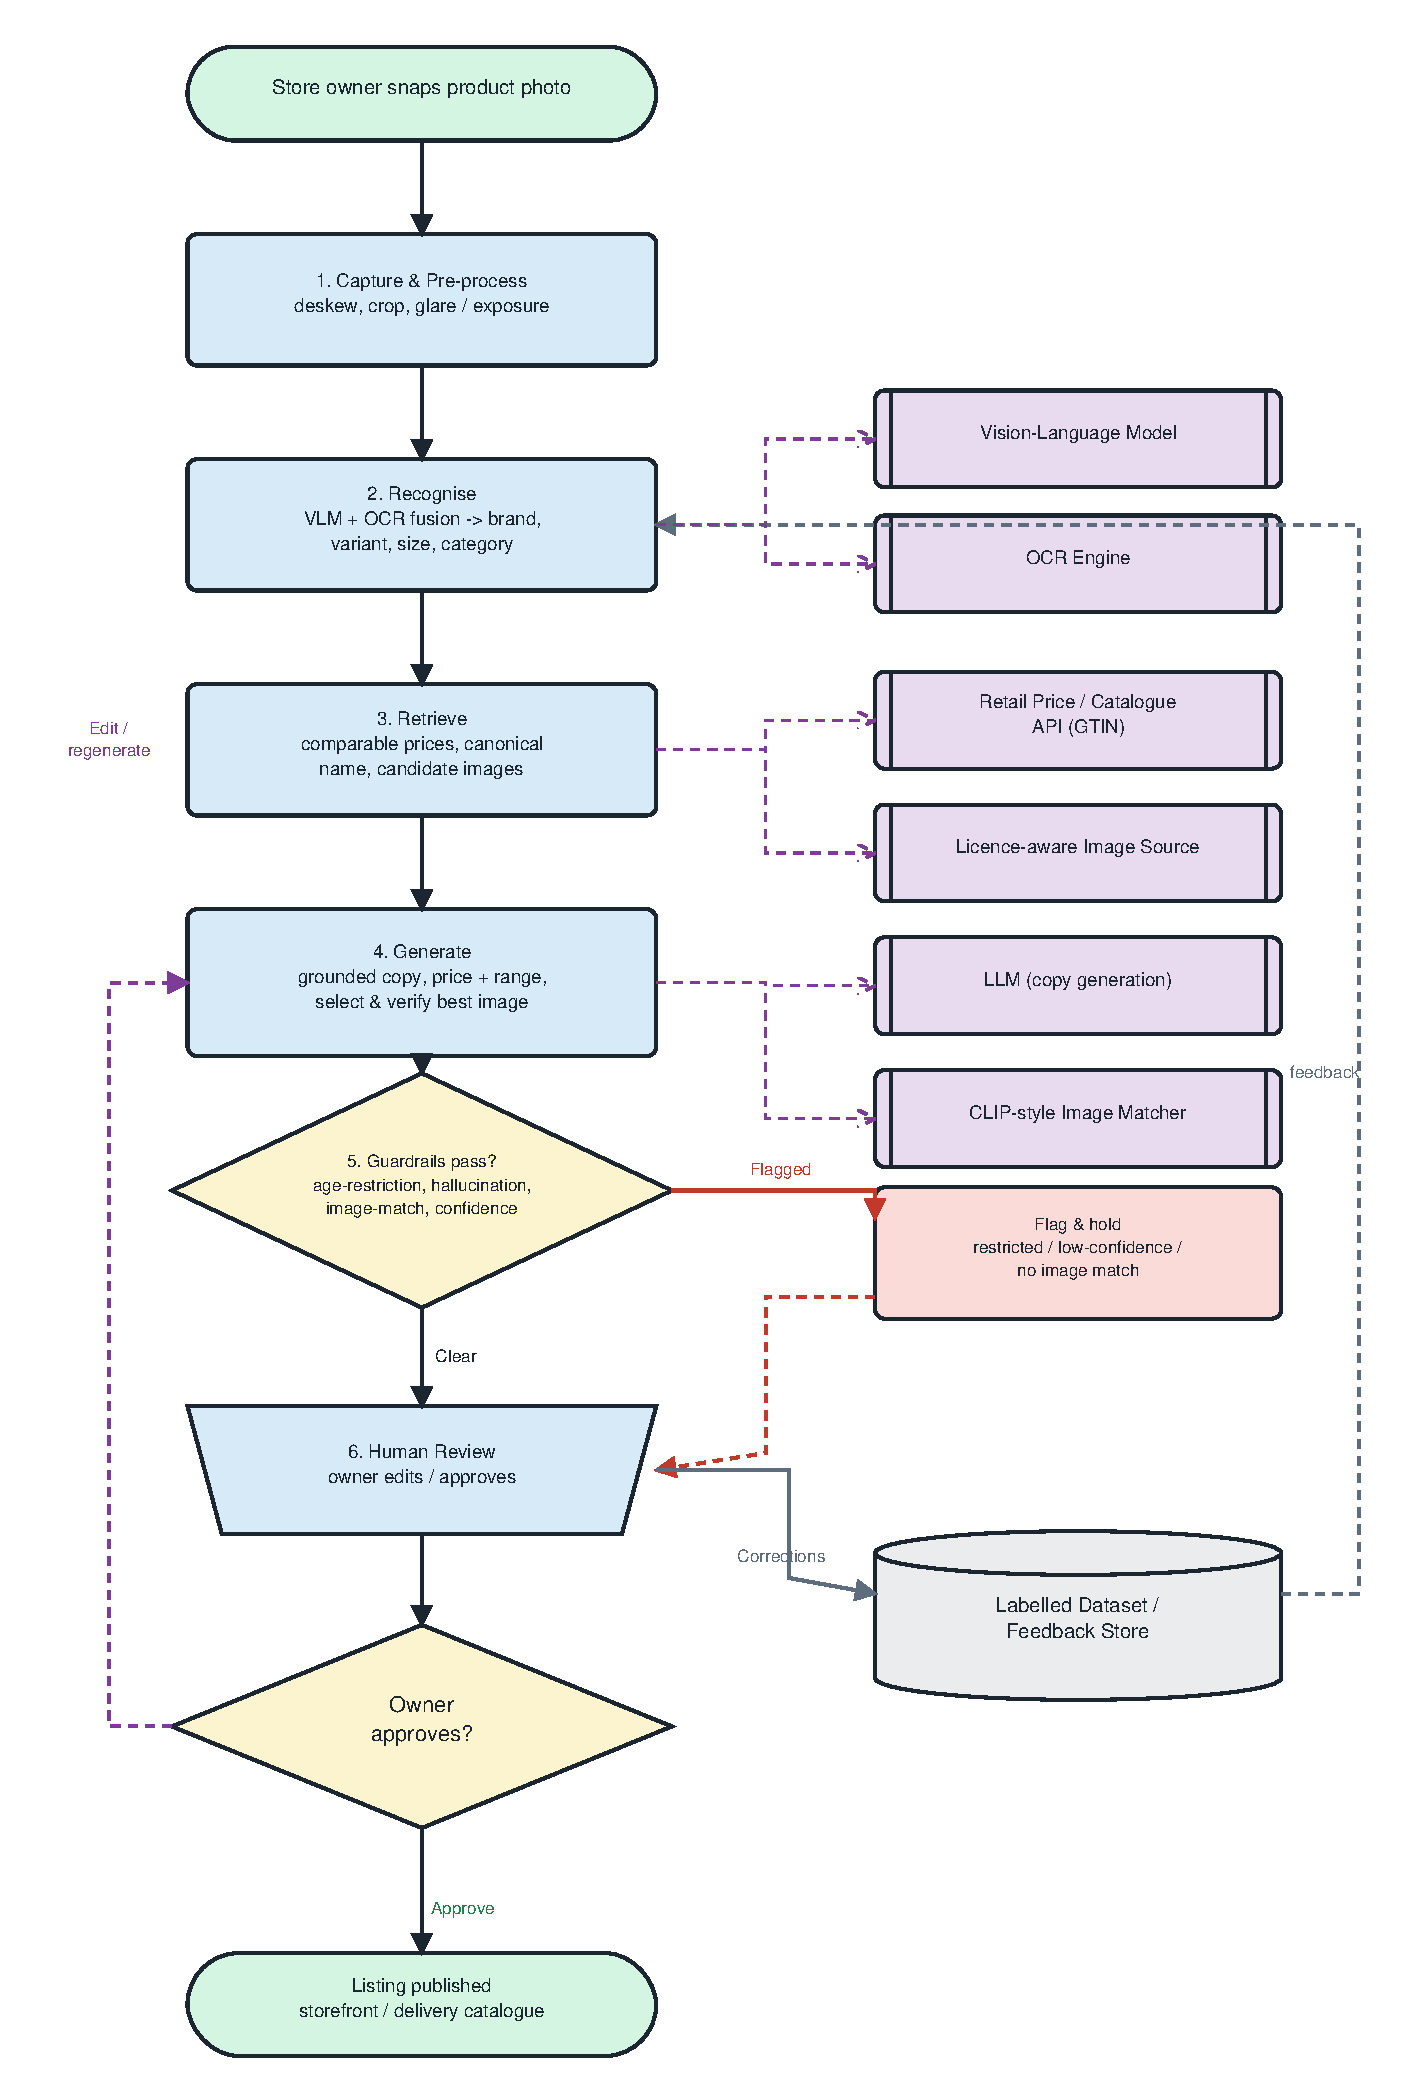
\includegraphics[height=7in]{architecture.pdf}}
\caption{Snap-to-Sell end-to-end architecture.}
\label{fig:processflow_appendix}
\end{figure}

\clearpage

\begin{figure*}[h]
\centering
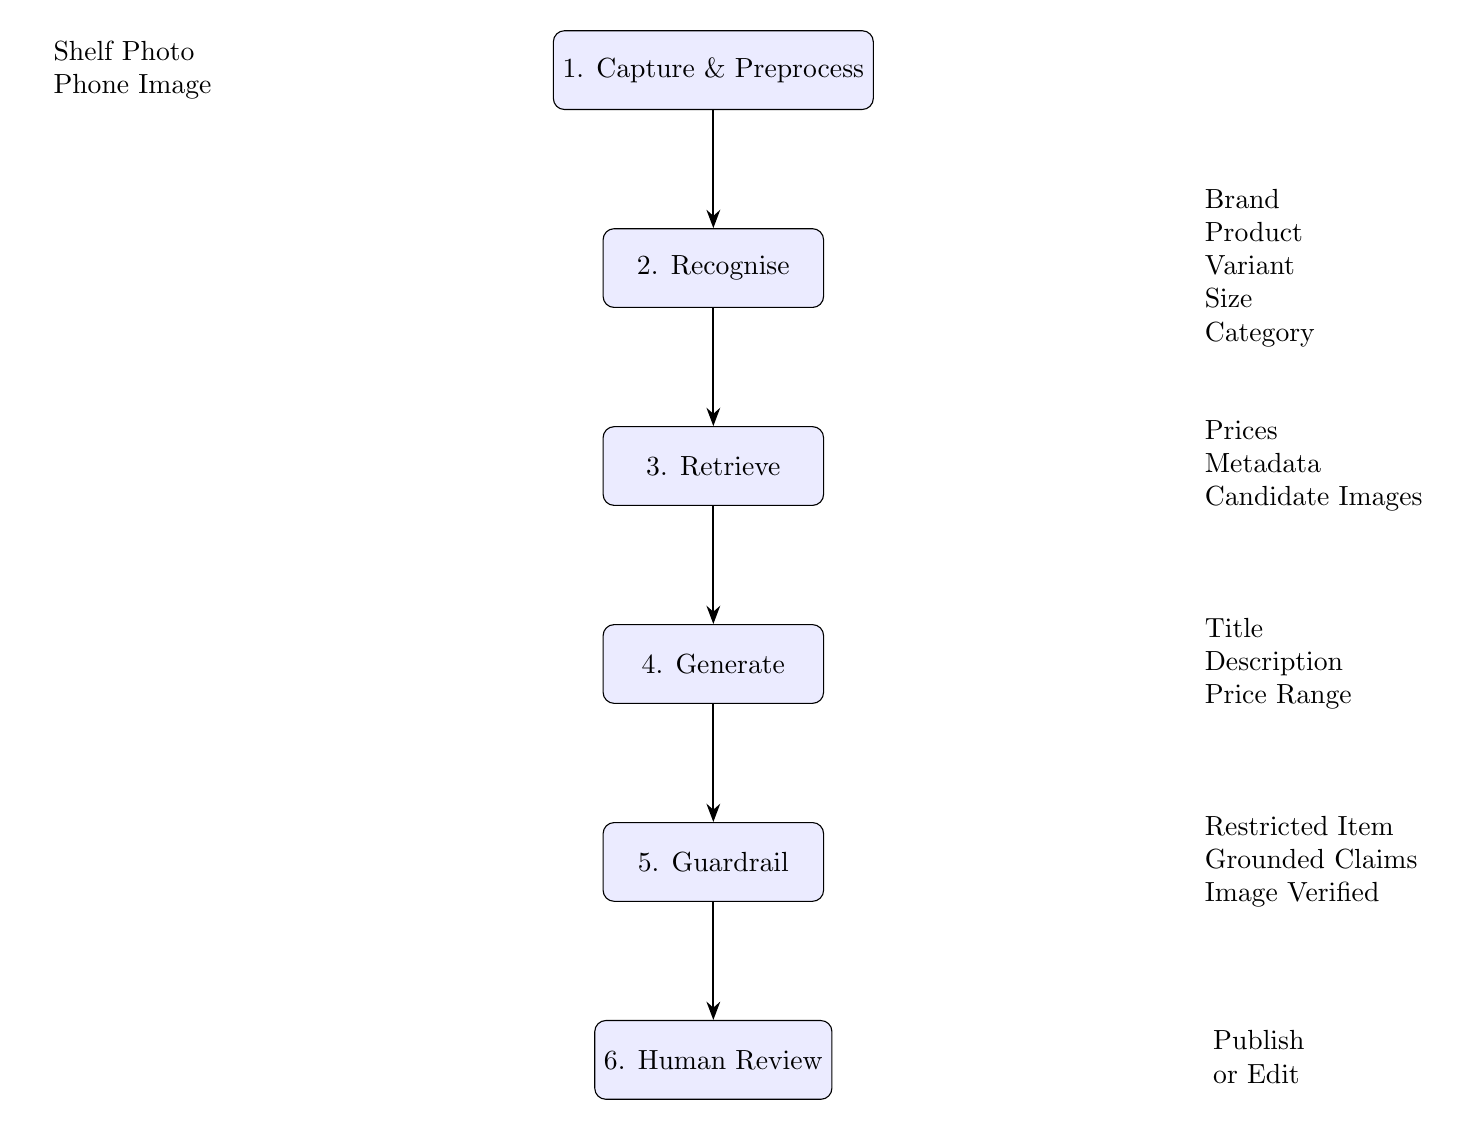
\begin{tikzpicture}[node distance=1.5cm]

\node (capture) [block] {1. Capture \& Preprocess};
\node (recognise) [block, below=of capture] {2. Recognise};
\node (retrieve) [block, below=of recognise] {3. Retrieve};
\node (generate) [block, below=of retrieve] {4. Generate};
\node (guardrail) [block, below=of generate] {5. Guardrail};
\node (review) [block, below=of guardrail] {6. Human Review};

\draw [arrow] (capture) -- (recognise);
\draw [arrow] (recognise) -- (retrieve);
\draw [arrow] (retrieve) -- (generate);
\draw [arrow] (generate) -- (guardrail);
\draw [arrow] (guardrail) -- (review);

\node[left=4cm of capture] {
\begin{tabular}{l}
Shelf Photo\\
Phone Image
\end{tabular}
};

\node[right=4.5cm of recognise] {
\begin{tabular}{l}
Brand\\
Product\\
Variant\\
Size\\
Category
\end{tabular}
};

\node[right=4.5cm of retrieve] {
\begin{tabular}{l}
Prices\\
Metadata\\
Candidate Images
\end{tabular}
};

\node[right=4.5cm of generate] {
\begin{tabular}{l}
Title\\
Description\\
Price Range
\end{tabular}
};

\node[right=4.5cm of guardrail] {
\begin{tabular}{l}
Restricted Item\\
Grounded Claims\\
Image Verified
\end{tabular}
};

\node[right=4.5cm of review] {
\begin{tabular}{l}
Publish\\
or Edit
\end{tabular}
};

\end{tikzpicture}

\caption{Process flow: capture, recognise (VLM + OCR), retrieve
(price, canonical name, candidate images), generate, guardrails, human review,
and publish}
\label{fig:architecture_appendix}
\end{figure*}

\section{Data Flow}

Figure~\ref{fig:dataflow} shows the data-flow view of artifacts passed
between stages, from raw photo to published catalogue entry, with external
datastores feeding retrieval, and Figure~\ref{fig:dataflow_appendix}
illustrates the artifacts exchanged between pipeline stages in more detail.

\begin{figure*}[h]
\centering

\resizebox{\textwidth}{!}{%
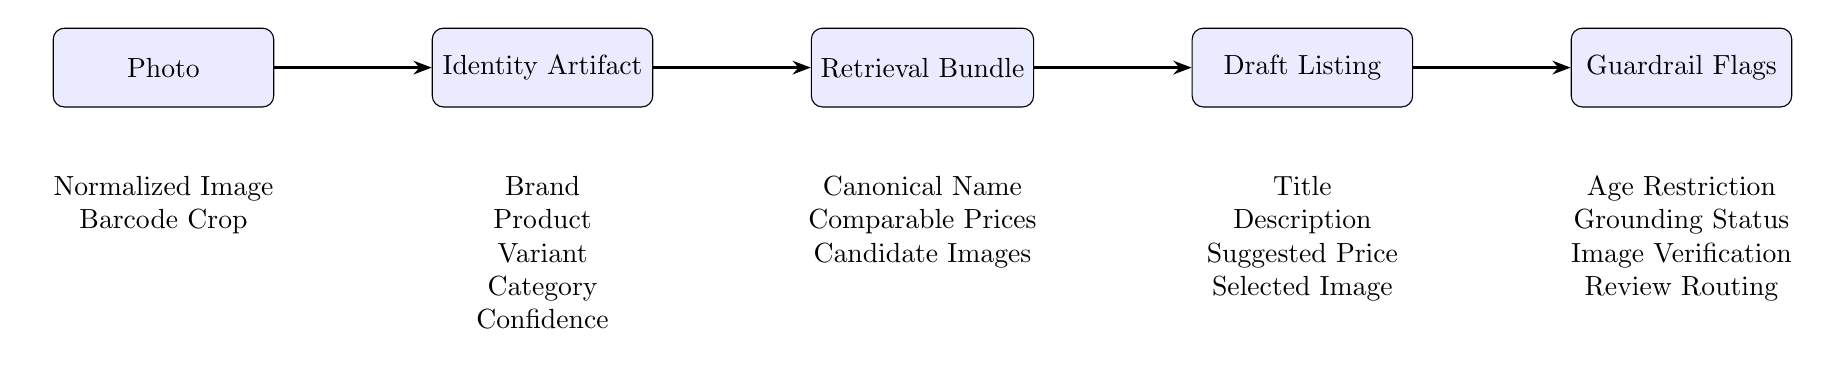
\begin{tikzpicture}[node distance=2cm]

\node (photo) [block] {Photo};
\node (identity) [block, right=of photo] {Identity Artifact};
\node (bundle) [block, right=of identity] {Retrieval Bundle};
\node (draft) [block, right=of bundle] {Draft Listing};
\node (flags) [block, right=of draft] {Guardrail Flags};

\draw [arrow] (photo) -- (identity);
\draw [arrow] (identity) -- (bundle);
\draw [arrow] (bundle) -- (draft);
\draw [arrow] (draft) -- (flags);

\node[below=0.7cm of photo] {
\begin{tabular}{c}
Normalized Image\\
Barcode Crop
\end{tabular}
};

\node[below=0.7cm of identity] {
\begin{tabular}{c}
Brand\\
Product\\
Variant\\
Category\\
Confidence
\end{tabular}
};

\node[below=0.7cm of bundle] {
\begin{tabular}{c}
Canonical Name\\
Comparable Prices\\
Candidate Images
\end{tabular}
};

\node[below=0.7cm of draft] {
\begin{tabular}{c}
Title\\
Description\\
Suggested Price\\
Selected Image
\end{tabular}
};

\node[below=0.7cm of flags] {
\begin{tabular}{c}
Age Restriction\\
Grounding Status\\
Image Verification\\
Review Routing
\end{tabular}
};

\end{tikzpicture}%
}

\caption{Data artifacts exchanged between pipeline stages.}
\label{fig:dataflow_appendix}
\end{figure*}


\begin{figure}[h]
\centering
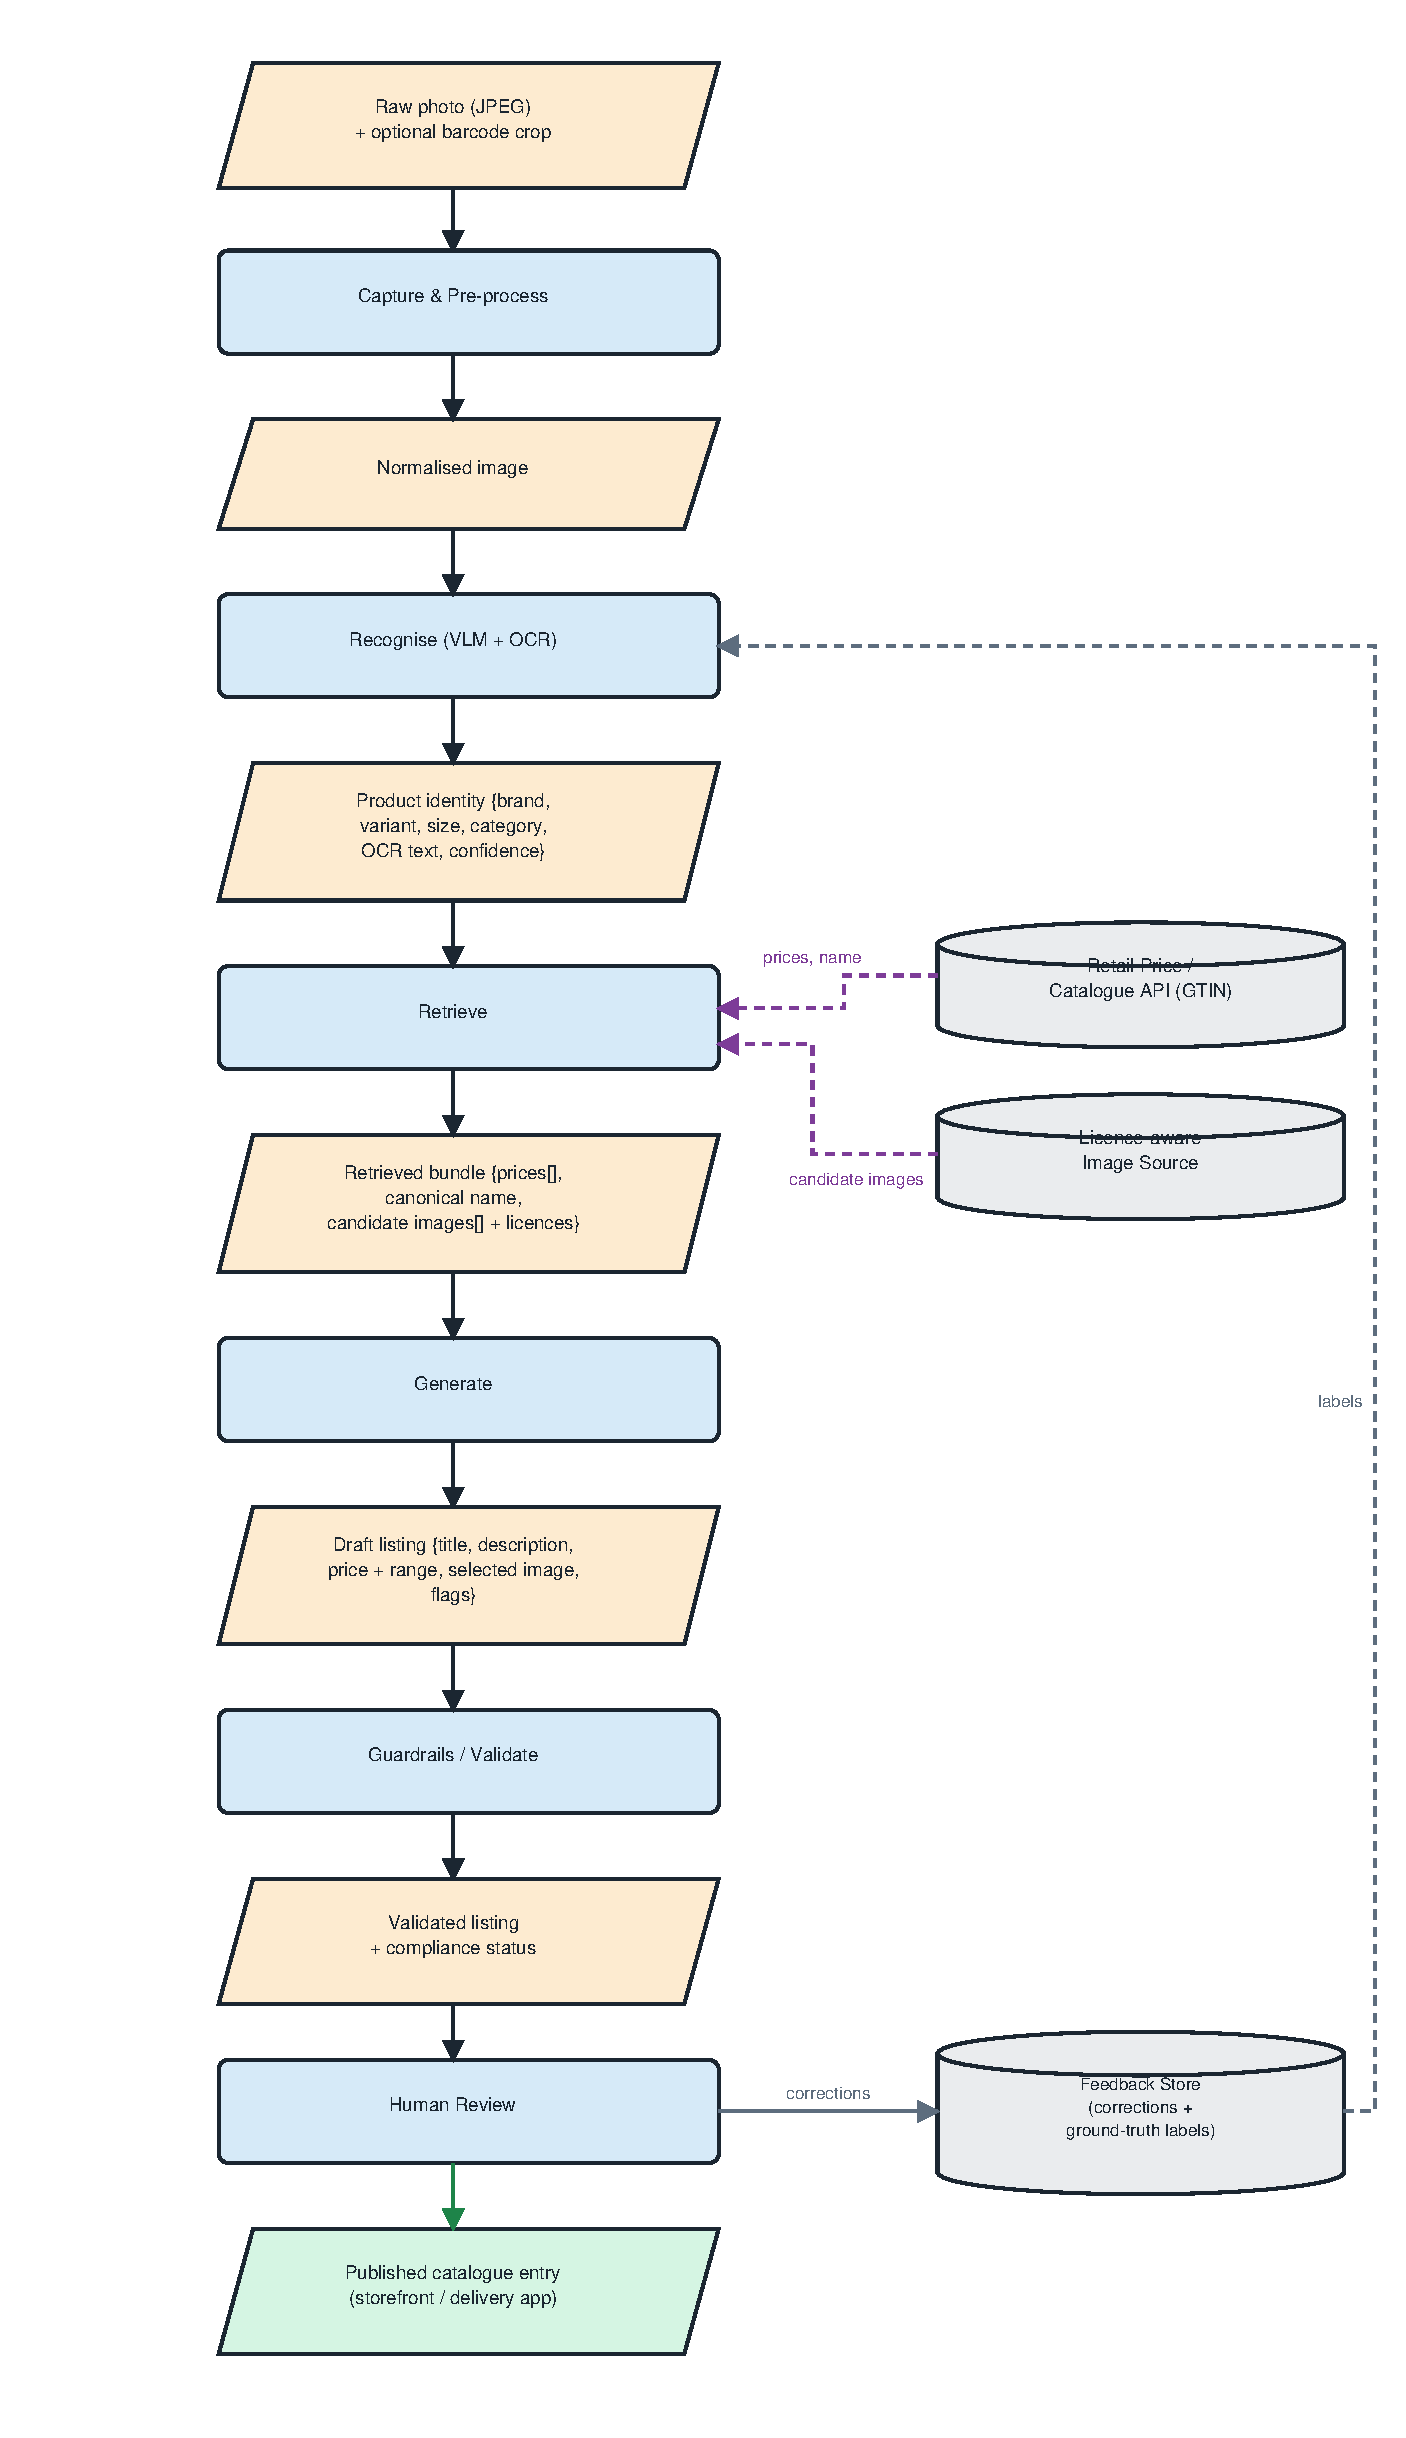
\includegraphics[height=6.5in]{dataflow.pdf}
\caption{Data-flow view: artifacts passed between stages, from raw photo to
published catalogue entry, with external datastores feeding retrieval.}
\label{fig:dataflow}
\end{figure}


\clearpage

\section{Supporting Tables}

\begin{table}[h]
\caption{Technology Stack}
\label{tab:stack_appendix}
\centering
\begin{tabular}{ll}
\toprule
Component & Technology \\
\midrule
Frontend & Streamlit \\
Preprocessing & OpenCV \\
OCR & PaddleOCR \\
Recognition & GPT-4o-mini \\
Retrieval & OFF / OPF / Open Prices \\
Image Matching & CLIP + pHash \\
Generation & Structured-output LLM \\
Guardrails & Rule-Based Validation \\
Reporting & HTML Trace Layer \\
\bottomrule
\end{tabular}
\end{table}

\begin{table*}[h]
\caption{Artifacts Exchanged Between Pipeline Stages}
\label{tab:artifacts_appendix}
\centering
\small
\begin{tabular}{lll}
\toprule
Stage & Artifact & Contents \\
\midrule
Capture & Photo & Normalized image, barcode crop \\
Recognition & Identity Object & Brand, product, variant, size, category, confidence \\
Retrieval & Retrieval Bundle & Canonical name, comparable prices, candidate images \\
Generation & Draft Listing & Title, description, suggested price, selected image \\
Guardrail & Validation Flags & Age restriction, grounding status, review route \\
Review & Final Listing & Approved publication-ready listing \\
\bottomrule
\end{tabular}
\end{table*}

\begin{table}[h]
\caption{Major Failure Categories}
\label{tab:failures_appendix}
\centering
\begin{tabular}{ll}
\toprule
Failure Type & Impact \\
\midrule
Multipack Retrieval & Incorrect pricing \\
Look-Alike Products & Wrong comparables \\
Regional Variants & Ambiguous matches \\
Restricted Products & Reduced retrieval coverage \\
Low Resolution Images & Prevented image replacement \\
\bottomrule
\end{tabular}
\end{table}

\end{document}
